\documentclass[10pt,twocolumn,letterpaper]{article}

% ---------------------------------------------------------------- packages
\usepackage[T1]{fontenc}
\usepackage[utf8]{inputenc}
\usepackage{mathptmx}
\usepackage[scaled=0.92]{helvet}
\usepackage{courier}
\usepackage[margin=0.75in,columnsep=0.28in]{geometry}
\usepackage{microtype}
\usepackage{amsmath,amssymb}
\usepackage{booktabs}
\usepackage{tabularx}
\usepackage{array}
\usepackage{multirow}
\usepackage{graphicx}
\usepackage{xcolor}
\usepackage{enumitem}
\usepackage[font=small,labelfont=bf,skip=4pt]{caption}
\usepackage{algorithm}
\usepackage{algpseudocode}
\usepackage{tikz}
\usetikzlibrary{arrows.meta,positioning,fit,backgrounds,calc}
\usepackage{url}
\usepackage[hidelinks]{hyperref}
\usepackage[capitalise,noabbrev]{cleveref}
\usepackage{balance}

% ---------------------------------------------------------------- macros
\newcommand{\sys}{Fabric}
\newcommand{\code}[1]{\texttt{\small #1}}
\newcommand{\ev}[1]{\textsc{#1}}            % evidence class label
\newcommand{\Measured}{\ev{measured}}
\newcommand{\PointInTime}{\ev{point-in-time}}
\newcommand{\Simulated}{\ev{simulated}}
\newcommand{\DevOnly}{\ev{dev-only}}
\newcommand{\Designed}{\ev{designed}}
\newcommand{\Tested}{\ev{tested}}
\newcommand{\repourl}{\texttt{[repository URL withheld; to be added]}}
\definecolor{cfg}{HTML}{7451A6}
\definecolor{gen}{HTML}{2878B5}
\definecolor{ink}{HTML}{17202A}
\definecolor{soft}{HTML}{F4F7FA}
\setlist{leftmargin=*,itemsep=1pt,topsep=2pt,parsep=0pt}
\renewcommand{\arraystretch}{1.08}
\setlength{\tabcolsep}{4pt}
\algrenewcommand\algorithmicrequire{\textbf{Input:}}
\algrenewcommand\algorithmicensure{\textbf{Output:}}

\title{\textbf{Fabric: Two-Clock Governance for Managed,\\Multi-Stamp, Agentic LLM Serving}}
\author{Author Name\\Affiliation\\\texttt{email}}
\date{November 2026}

\begin{document}
\maketitle

% ================================================================= abstract
\begin{abstract}
A managed language-model service runs on two clocks. The \emph{configuration clock} moves
account intent through placement, cluster reconciliation and minutes-long model cold starts;
the \emph{generation clock} authenticates, admits and streams a request token by token. In
earlier work on \sys{}, an implemented Kubernetes-based serving platform, we argued that
coupling the two clocks makes every stream depend on a distant database, and derived
invariants that keep authorization at the serving edge and require evidence before any
acknowledgement or destructive transition. This paper extends that account to three
developments that stress the split: a single edge endpoint in front of many independently
operated GPU and TPU ``stamps''; prefix-cache-aware routing; and agentic requests, in which
one task is a sequence of model calls with tools, budgets and structured output. We make
one organising rule explicit: \emph{state lives with the clock that reads it on the hot
path}. Configuration state reaches serving components only as versioned, cached snapshots
(routing tables, signing keys, route sets); generation state (prefix caches, run budgets,
traces, in-flight leases) stays where it is consumed, and the affinity requirements of the
edge follow from where that state lives. We describe the edge gateway, a tokenizer-free
prefix-aware router with a load bound, gateway-side agent governance (run budgets,
content-free traces, and a tool-call guard that repairs invalid tool calls and re-asks
without tools when a model ignores a requested JSON schema), and an outbound-only stamp
agent with one-command bootstrap across NVIDIA T4, A10 and RTX PRO 6000 (Blackwell) GPUs,
with Cloud TPU support implemented but not yet validated on hardware. The evaluation is
deliberately classified by evidence type. Against simulated model hosts behind the
production gateway, prefix-aware routing with a 1.1 load bound reduced median time to
first token by 29--39\% relative to least-in-flight below saturation while keeping its
tail, and reached 75--79\% of the reachable cache-hit rate when shared prompts exceeded one
host's cache, against 19--38\% for the alternatives. Point-in-time live checks show a
96\,GiB Blackwell stamp enrolled by the bootstrap serving a 35B-parameter FP8
mixture-of-experts model with a 64K context, and the gateway's structured-output repair
passing 3/3 trials and an 8-check agent-SDK smoke test. We report no hardware throughput
claims, and we list the defects and unvalidated paths the evidence exposes.
\end{abstract}

\noindent\textbf{Keywords:} LLM serving, control planes, edge routing, prefix caching,
LLM agents, tool calling, multi-tenancy, Kubernetes, heterogeneous accelerators.

% ================================================================= introduction
\section{Introduction}
\label{sec:intro}

Serving large language models (LLMs) as a managed service combines two systems that run
at very different rates. An administrative system changes accounts, keys, deployments,
placements and releases; its unit of progress is a reconciled configuration, and a single
step can take many minutes because a GPU must be scheduled, a multi-gigabyte image pulled,
weights loaded and an engine warmed up. A real-time system authenticates a prompt, admits
it, attaches it to a model process and extends a sequence token by token; its unit of
progress is a request or a token, measured in milliseconds, and a stream cannot pause while
a central database recovers. Earlier work on \sys{}~\cite{priorpaper} named these the
\emph{configuration clock} and the \emph{generation clock} and derived three invariants:
authority should not accumulate in one credential domain; authorization is decided at the
serving edge from local state; and an acknowledgement or destructive transition must follow
durable or directly observed evidence.

That analysis covered one Kubernetes cluster (a ``stamp''~\cite{stamps}) with one model
per T4 GPU and one OpenAI-compatible request at a time. Three developments since then put
pressure on the split:

\begin{enumerate}
  \item \textbf{One endpoint, many stamps.} Customers deploy models on several stamps
  (an AKS GPU pool, a k3s VM with one large GPU, a TPU VM) and do not want to know which
  URL serves which model. The obvious solution, routing inference through the control
  plane, re-couples the clocks.
  \item \textbf{Cache-aware placement of requests.} Engines with paged KV
  caches~\cite{vllm,sglang} skip prefill for a prompt prefix they already hold. Where a
  request lands therefore decides its cost, but the gateway cannot see an engine's cache
  and does not tokenize.
  \item \textbf{Agentic requests.} An agent is a loop of model calls interleaved with tool
  executions~\cite{react,toolformer}. Per-request controls cannot express ``this task may
  spend 20{,}000 tokens or 8 steps'', and small open models frequently emit undeclared
  tools, schema-violating arguments, or prose where a JSON object was requested.
\end{enumerate}

Each development introduces state. The question this paper answers is \emph{where that
state may live} without coupling the clocks or weakening the invariants. Our answer is a
single rule: \textbf{state lives with the clock that reads it on the hot path.}
Configuration state is produced on the configuration clock and reaches serving components
only as versioned, cached, monotone snapshots that the generation clock can consume while
the producer is down. Generation state is produced and consumed on the generation clock and
stays where it is consumed; any component that routes requests must then provide the
\emph{affinity} that state requires. This rule explains, for example, why \sys{}'s edge
gateway meters nothing, why agent runs pin strictly to one stamp while sessions pin only
softly, and why the prefix index is a process-local guess rather than a replicated
structure.

\paragraph{Contributions.}
\begin{itemize}
  \item A \textbf{state-placement extension of the two-clock model} (\cref{sec:model})
  that classifies every piece of serving state by producing and consuming clock, and
  derives a fourth invariant: affinity requirements follow generation-state locality.
  \item The \textbf{design of an edge tier} (\cref{sec:edge}) that provides one inference
  URL across heterogeneous stamps while preserving local authorization (tokens are verified
  at the edge and again at the stamp), keeping the control plane off the request path, and
  never replaying a request that may have reached a stamp.
  \item A \textbf{tokenizer-free, prefix-aware routing strategy with a load bound}
  (\cref{sec:prefix}) and its evaluation against simulated hosts behind the production
  gateway, including a bound-sensitivity study (\cref{sec:eval-routing}).
  \item \textbf{Gateway-side agent governance} (\cref{sec:agents}): task-level run
  budgets, content-free run traces, a tool-call guard that repairs invalid calls and
  enforces a requested JSON schema on a final answer when the engine does not, a
  server-side tool loop and a bounded model cascade, all metered honestly.
  \item \textbf{Heterogeneous stamp enrollment} (\cref{sec:config}): an outbound-only agent
  that measures capacity and pushes status, activity and serving metrics, and a
  one-command bootstrap with preflight checks spanning three NVIDIA GPU generations and
  Cloud TPU.
  \item An \textbf{evidence-classified evaluation} (\cref{sec:eval}) that separates
  simulated, point-in-time, dated, development-only and designed-but-unvalidated claims,
  and reports defects the evidence exposed.
\end{itemize}

This is an experience and design paper about an implemented system. Its quantitative
results are limited: the routing study uses simulated hosts, and live checks are single
observations. \Cref{sec:eval-plan} states the evaluation that would close the gap.

% ================================================================= background
\section{Background and Related Work}
\label{sec:related}

\paragraph{Engines and schedulers.}
Orca introduced iteration-level scheduling for generative transformers~\cite{orca}; vLLM's
PagedAttention manages KV memory in pages and enables sharing~\cite{vllm}. Sarathi-Serve
chunks prefill to bound decode stalls~\cite{sarathi}; DistServe and Splitwise disaggregate
prefill and decode~\cite{distserve,splitwise}. Llumnix migrates requests between engine
instances at runtime~\cite{llumnix}. Clockwork obtains predictable latency by centralising
scheduling decisions~\cite{clockwork}, and AlpaServe multiplexes models with model
parallelism~\cite{alpaserve}. \sys{} uses vLLM as its engine and deliberately does not
replace its scheduler: our concerns are identity, placement, routing between engine
instances, rollout safety, metering and agent governance around the engine. Llumnix-style
migration is incompatible with \sys{}'s rule that a stream is pinned after its first byte
(\cref{sec:retry}).

\paragraph{Prefix reuse and cache-aware routing.}
SGLang's RadixAttention keeps a radix tree of KV-cached prefixes within an
engine~\cite{sglang}; Preble schedules prompts across GPUs using prefix sharing and load
together~\cite{preble}. \sys{}'s router is closer to Preble's goal but operates with less
information: it sees only request bytes, not tokens or the engine's eviction decisions, so
it hashes byte blocks and bounds load in the manner of consistent hashing with bounded
loads~\cite{karger,boundedloads}. Rendezvous hashing~\cite{rendezvous} provides \sys{}'s
explicit session and run affinity.

\paragraph{Model serving systems and cold start.}
Clipper and INFaaS provide model-agnostic serving front ends and automated model
selection~\cite{clipper,infaas}; \sys{}'s \code{model: auto} and cascade
(\cref{sec:cascade}) are deliberately simple, explainable relatives of model selection and
of LLM cascades such as FrugalGPT and RouteLLM~\cite{frugalgpt,routellm}. ServerlessLLM
attacks LLM cold start with fast checkpoint loading~\cite{serverlessllm}; our cold-start
data (\cref{sec:eval-coldstart}) show that, on T4, engine profiling and warmup and GPU
availability dominate weight loading, so cold start is a configuration-clock cost that
placement and rollout must budget for.

\paragraph{LLM applications and agents.}
ReAct and Toolformer established tool-using language agents~\cite{react,toolformer};
Gorilla studied API-call accuracy~\cite{gorilla}. On the serving side, Parrot exposes
application structure to the server~\cite{parrot}, and InferCept handles the KV state of
requests paused for tool calls~\cite{infercept}. Constrained decoding enforces output
grammars inside the engine~\cite{outlines}. \sys{} is complementary: it governs agent loops
at the gateway with budgets, traces and validation, and it compensates for an observed gap
in which the engine does not apply a requested \code{response\_format} while tools are
offered with automatic tool choice (\cref{sec:guard}).

\paragraph{Control planes and isolation.}
\sys{}'s reconciliation follows the Kubernetes controller and operator
patterns~\cite{k8scontroller,k8soperator,borgomegak8s} descended from Borg~\cite{borg}.
Credentials are JWTs~\cite{rfc7519,rfc8725} verified against cached JWKS~\cite{rfc7517},
issued by exchange~\cite{rfc8693}. Tenant data in the control plane is protected by forced
PostgreSQL row-level security~\cite{pgrls}. The invariants resemble resource-centric
guidance in NIST SP~800-207~\cite{nistzt}, but we make narrower, testable claims.
Hosted code execution can use Firecracker microVMs~\cite{firecracker} or a gVisor
runtime~\cite{gvisor}.

% ================================================================= model
\section{System Model: Clocks and State Placement}
\label{sec:model}

\subsection{Two clocks}
Let $C(t)$ be central intent at administrative time $t$. Intent passes through an
agent-applied local set $A$, an operator observation $O$ and a gateway route configuration
$R$, each by asynchronous, repeated reconciliation: $C \rightarrow A \rightarrow O
\rightarrow R$. A request arriving at generation time $\tau$ is decided from a local tuple
\begin{equation}
  Q(\tau) = \langle K_\tau, R_\tau, L_\tau, B_\tau, S_\tau \rangle
\end{equation}
of cached verification keys $K$, account-scoped routes $R$, admission state $L$, backend
health and in-flight state $B$, and a durable usage spool $S$---never from a synchronous
read of $C(t)$~\cite{priorpaper}. Independence is bounded: an unknown key identifier, an
unhealthy spool or an unavailable local limiter refuses new work rather than inventing
authority.

\subsection{State placement}
The developments in \cref{sec:intro} add state to $Q$. We classify each item by the clock
that \emph{produces} it and the clock that \emph{reads it on the hot path}
(\cref{tab:state}). Three cases arise.

\textbf{Configuration-produced, generation-read} state (routing tables, keys, route
sets, cascade tiers) is published as a \emph{snapshot} with a monotone revision. A consumer
(i) caches the last good snapshot, including on disk, (ii) refuses a snapshot older than
the one it holds, and (iii) keeps serving from the cache while the producer is
unavailable. A snapshot conveys permission (ownership, placement), never an
acknowledgement of anything the generation clock has done.

\textbf{Generation-produced, generation-read} state (prefix caches, run budgets and
traces, in-flight leases, sandbox sessions) stays local to the component that consumes it.
It is not replicated, so its correctness depends on requests that share it reaching the
same component. A router in front of that state therefore inherits an \emph{affinity
obligation} whose strength matches the cost of losing the state: \emph{strict} when losing
it changes semantics (a budget would reset), \emph{soft} when it only changes cost (a cache
miss).

\textbf{Generation-produced, configuration-read} state (usage records, activity events,
serving metrics, host logs) flows outward asynchronously, is spooled locally, and is
deleted only after central acknowledgement.

\begin{table}[t]
\centering
\caption{Serving state by producing and hot-path consuming clock (C = configuration,
G = generation) and how \sys{} places it.}
\label{tab:state}
\small
\begin{tabularx}{\columnwidth}{@{}l c X@{}}
\toprule
State & Prod.$\to$read & Placement and obligation \\
\midrule
Routing table (edge) & C$\to$G & Polled snapshot, ETag, monotone revision, disk cache \\
JWKS & C$\to$G & Cached; refetch on unknown \code{kid}, rate-limited \\
Stamp route set & C$\to$G & Rendered by operator; last good kept on error \\
In-flight leases & G$\to$G & Per gateway; drain evidence for rollouts \\
Prefix index & G$\to$G & Per gateway process; soft affinity \\
Run budget, trace & G$\to$G & Per stamp gateway, in memory; strict affinity \\
Sandbox session & G$\to$G & Keyed by (account, run); follows the run \\
Usage records & G$\to$C & Durable spool; delete after central ack \\
Activity, metrics & G$\to$C & Bounded buffers; deduplicated by event id \\
\bottomrule
\end{tabularx}
\end{table}

\subsection{Invariants}
The earlier invariants carry over unchanged~\cite{priorpaper}; state placement adds a
fourth.
\begin{description}[leftmargin=0pt,font=\normalfont\bfseries]
  \item[I1 Non-aggregation of authority.] Central synchronization, cluster mutation,
  request serving, routing-table reading and telemetry export hold distinct credentials.
  \item[I2 Local authorization.] Every serving tier verifies audience, scope and account
  ownership from cached state; none consults the control plane per request.
  \item[I3 Evidence before transition.] Watermarks advance, leases are deleted and old
  releases are destroyed only after durable writes or direct observation.
  \item[I4 Affinity follows locality.] A router must deliver every request that reads a
  piece of generation state to the component that holds it, strictly if loss changes
  semantics and softly if it changes only cost; it must not duplicate side effects
  (metering, limits) that the holder already performs.
\end{description}
I4 has a corollary for retries: a router may move a request only while it can prove the
holder never received it, because the holder's state (and the request's cost) may already
have changed.

% ================================================================= architecture
\section{Architecture Overview}
\label{sec:arch}

\Cref{fig:arch} shows the components. The \textbf{control plane} (Python, FastAPI,
PostgreSQL) owns accounts, memberships, API keys, deployments, placements, stamp enrollment,
audit records, observed status and aggregated usage. It issues short-lived RS256 JWTs with
separate audiences for control and inference. The \textbf{edge gateway} is a separate
service, built from the data-plane image, that fronts all stamps with one inference URL.
Each \textbf{stamp} is a failure and serving domain containing an \emph{agent} that
enrolls, polls desired state and pushes status outbound; an \emph{operator} that
reconciles a \code{FabricModelDeployment} custom resource into model-host workloads and
gateway routes; a stamp \emph{gateway} that verifies tokens, admits, routes, streams,
meters and governs agent runs; and a \emph{collector} that exports spooled usage. Model
hosts run vLLM. A web console reads only the control plane.

\begin{figure*}[t]
\centering
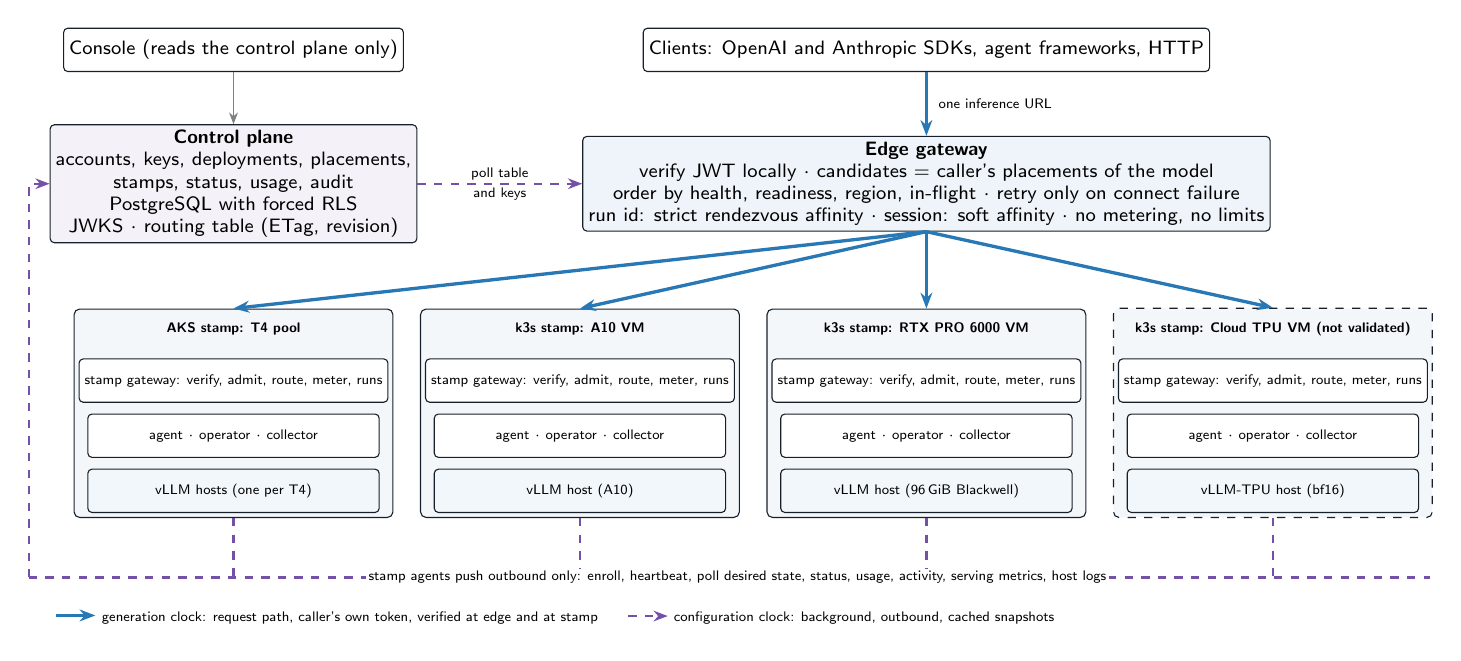
\begin{tikzpicture}[
  font=\sffamily\scriptsize,
  x=1mm, y=1mm,
  comp/.style={draw=ink, rounded corners=1.5pt, fill=white, align=center, inner sep=2pt, minimum height=5.5mm},
  inner/.style={comp, minimum width=37mm, font=\sffamily\tiny},
  gen/.style={-{Stealth[length=2mm]}, very thick, draw=gen},
  cfg/.style={-{Stealth[length=1.8mm]}, thick, dashed, draw=cfg},
  cfgl/.style={thick, dashed, draw=cfg},
  lbl/.style={font=\sffamily\tiny, fill=white, inner sep=1pt, align=center}
]
% top rows
\node[comp, minimum width=60mm] (clients) at (112,0) {Clients: OpenAI and Anthropic SDKs, agent frameworks, HTTP};
\node[comp, minimum width=30mm] (console) at (24,0) {Console (reads the control plane only)};
\node[comp, minimum width=44mm, fill=cfg!8] (cp) at (24,-17)
  {\textbf{Control plane}\\accounts, keys, deployments, placements,\\stamps, status, usage, audit\\PostgreSQL with forced RLS\\JWKS $\cdot$ routing table (ETag, revision)};
\node[comp, minimum width=86mm, fill=gen!8] (edge) at (112,-17)
  {\textbf{Edge gateway}\\verify JWT locally $\cdot$ candidates = caller's placements of the model\\order by health, readiness, region, in-flight $\cdot$ retry only on connect failure\\run id: strict rendezvous affinity $\cdot$ session: soft affinity $\cdot$ no metering, no limits};
\draw[gen] (clients) -- node[lbl,right=1mm]{one inference URL} (edge);
\draw[-{Stealth[length=1.5mm]}, thin, draw=gray] (console) -- (cp);
\draw[cfg] (cp.east) -- node[lbl,above]{poll table}node[lbl,below]{and keys} (edge.west);

% stamps
\foreach \i/\x/\title/\host in {1/24/AKS stamp: T4 pool/vLLM hosts (one per T4),
                               2/68/k3s stamp: A10 VM/vLLM host (A10),
                               3/112/k3s stamp: RTX PRO 6000 VM/vLLM host (96\,GiB Blackwell),
                               4/156/k3s stamp: Cloud TPU VM (not validated)/vLLM-TPU host (bf16)} {
  \node[inner] (g\i) at (\x,-42) {stamp gateway: verify, admit, route, meter, runs};
  \node[inner] (a\i) at (\x,-49) {agent $\cdot$ operator $\cdot$ collector};
  \node[inner, fill=gen!6] (m\i) at (\x,-56) {\host};
  \node[font=\sffamily\tiny\bfseries] (t\i) at (\x,-35.5) {\title};
}
\begin{scope}[on background layer]
  \foreach \i in {1,2,3} { \node[draw=ink, rounded corners=2pt, fill=soft, inner sep=1.6pt, fit=(t\i)(g\i)(m\i)] (s\i) {}; }
  \node[draw=ink, dashed, rounded corners=2pt, fill=soft, inner sep=1.6pt, fit=(t4)(g4)(m4)] (s4) {};
\end{scope}
\foreach \i in {1,2,3,4} { \draw[gen] (edge.south) -- (s\i.north); }

% outbound bus
\draw[cfgl] (-2,-67) -- (176,-67);
\foreach \i in {1,2,3,4} { \draw[cfgl] (s\i.south) -- (s\i.south |- 0,-67); }
\draw[cfg] (-2,-67) -- (-2,-17) -- (cp.west);
\node[lbl] at (88,-67) {stamp agents push outbound only: enroll, heartbeat, poll desired state, status, usage, activity, serving metrics, host logs};

% legend
\node[font=\sffamily\tiny, anchor=west] at (0,-72)
  {\tikz{\draw[gen] (0,0) -- (5mm,0);} generation clock: request path, caller's own token, verified at edge and at stamp\qquad
   \tikz{\draw[cfg] (0,0) -- (5mm,0);} configuration clock: background, outbound, cached snapshots};
\end{tikzpicture}
\caption{\sys{} components and the two clocks. Solid arrows carry requests; each stamp
gateway verifies the caller's token again. Dashed arrows are background exchanges: the edge
polls a routing table and signing keys; every stamp agent initiates all exchanges with the
control plane (the control plane never connects into a stamp). The three GPU stamps match
the 16~November demonstration lineup (one model per GPU); the TPU path is implemented and
CI-checked but has not run on TPU hardware.}
\label{fig:arch}
\end{figure*}

% ================================================================= configuration clock
\section{The Configuration Clock}
\label{sec:config}

\subsection{Enrollment, measured capacity and placement}
A stamp begins with a short-lived, single-use, account-bound enrollment token. The control
plane consumes it atomically and issues separate agent and telemetry credentials (I1); the
agent persists its identity on a volume and reuses it after restart. Machine credentials
now rotate \emph{from the stamp}: the agent requests a new pair authorized by the
credential it replaces, and older credentials receive an expiry rather than immediate
revocation so the collector can switch files independently. Only the newest credential may
rotate (with a narrow exception for a lost reply), so a copied, superseded credential cannot
mint a fresh pair.

Placement is admission against \emph{measured} capacity. The agent reads node
allocatable counts and GPU labels (product, memory, compute capability), separates
Fabric-managed from foreign GPU requests, and reports a slot vector of how many $k$-GPU
replicas fit without splitting across nodes. The control plane refuses a placement that
cannot schedule with a typed reason (e.g.\ \code{insufficient\_free\_gpus}) instead of
returning success for a pod that would stay Pending. Accelerator classes constrain
placement: TPU classes go only to TPU stamps, GPU classes only to GPU stamps, and FP8
checkpoints are refused on TPU classes.

\subsection{Reconciliation and acknowledged rollouts}
The agent polls desired state after a durable watermark, rebuilds the complete assignment
set, publishes custom resources, and only then stores the new watermark; after losing its
rendered state it restarts from watermark zero (I3). The operator derives serving settings
from the weakest GPU in the pool, changing only settings the hardware makes impossible
(e.g.\ bfloat16 to float16 below compute capability 8.0). A release change starts a
candidate workload beside the active one; routes cut over only when the candidate has
concrete Ready endpoints, and the old workload is deleted only after the stamp gateway
reports the exact route revision loaded and zero in-flight requests on the old backends.
Without spare capacity the candidate stays Pending and the active release keeps serving:
the system degrades to ``no release'' rather than to silent downtime.

\subsection{Outbound observation}
Because the control plane never connects into a stamp, everything an operator or customer
needs to see is pushed by the agent over its own credential. Four streams exist, each
bounded and deduplicated:
\begin{itemize}
  \item \textbf{Host snapshots}: pod phase, readiness, the 20 most recent events and a
  sanitized tail of the model-host log (lines matching credential patterns are replaced),
  every 3\,s while a host is starting and every 30\,s once all are ready.
  \item \textbf{Activity events}: enrollment, accelerators measured, accelerator runtime
  allocatable, readiness, credential rotation, desired state applied, image pulls with
  duration and size, host failures. A buffer of 200 events survives disconnection; the
  control plane deduplicates by event id and stores them under forced RLS.
  \item \textbf{Serving metrics}: every 30\,s the agent scrapes the gateway, each vLLM
  host and the DCGM exporters, converts counters to deltas and histograms to per-bucket
  counts, and pushes one sample. The control plane merges samples into one-minute rows
  and computes percentiles from merged histograms, never from averaged percentiles; a
  missed report becomes a gap, not a dip.
  \item \textbf{Usage}: the gateway spools records; the collector leases batches and deletes
  them only after central acceptance, duplicate recognition or permanent rejection.
\end{itemize}
These streams are configuration-clock consumers of generation-clock data (\cref{tab:state})
and never sit on the request path.

\subsection{One-command bootstrap across accelerators}
A stamp on a single VM is created by one command that installs k3s, verifies the
accelerator runtime, configures TLS, stores the enrollment token in a Secret, installs the
stamp chart and images of one pinned release, and waits for enrollment. Re-running it
upgrades in place and keeps the stamp identity. Preflight checks turn common operator
errors into immediate, specific failures: the control-plane URL must serve a JWKS document
(rejecting, for example, the stamp's own hostname given by mistake); the token must have
the enrollment format; the stamp hostname's DNS record is compared with the VM's public
address from the cloud metadata service; and the accelerator is inspected. On NVIDIA hosts
the script reads product, memory and compute capability and selects float16 below compute
capability 8 and bfloat16 otherwise. On a VM without an NVIDIA driver it queries the GCP
metadata server for a TPU accelerator type, counts chip device nodes, refuses multi-host
slices, forces bfloat16, and advertises chips to Kubernetes as the \code{google.com/tpu}
extended resource with no device plugin. The operator then runs a vLLM TPU image with
tensor parallelism equal to the chips per replica and an XLA compilation cache beside the
weights. Long steps stream progress and a heartbeat so a cold image pull never looks like a
hang; an agent that has not enrolled within 15 minutes, or an image that cannot be pulled,
ends the script with a diagnosis.

\paragraph{Designed, not implemented: GPU sharing.} A replica holds whole GPUs today, so a
96\,GiB card serving a 35B-A3B FP8 model (about 37.5\,GB of weights) cannot also host a
small model. The accepted design uses device-plugin time-slicing with Fabric-enforced
memory shares: placement keeps the sum of fractions on each physical GPU at or below 0.95,
never mixes whole-GPU and shared deployments, reports physical rather than sliced GPU
counts, sets \code{-{}-gpu-memory-utilization} to the share times the stamp ceiling, starts
hosts on one GPU one at a time, and is restricted to single-GPU nodes because time-slicing
cannot bind a replica to a particular device. Isolation is cooperative; MIG is future work.

% ================================================================= generation clock
\section{The Generation Clock}
\label{sec:gen}

\subsection{Stamp request path}
The stamp gateway parses a bearer token, selects a cached key, verifies algorithm, issuer,
exact inference audience, time claims, account and \code{inference:invoke} scope, resolves
the model only among routes owned by that account, requires a healthy usage spool and
stamp-local limit authority, acquires admission and an in-flight lease, rewrites the public
alias to the internal release, strips caller-supplied identity headers, and proxies a
response or a pinned SSE stream. Admission combines a request bucket, an in-flight bound and
a token-rate bucket debited from metered usage, coordinated once per stamp across gateway
processes; limits are not global across stamps.

\paragraph{Protocol surfaces.} OpenAI chat completions, completions and Responses, and the
Anthropic Messages API~\cite{openaiapi,anthropicapi} share this path. Responses requests
are forwarded to engines that implement them, but the gateway enforces a stateless subset
(\code{store}, \code{background}, \code{previous\_response\_id} and \code{conversation} are
refused) because stored conversations would be generation state outside any affinity
guarantee. Messages requests are \emph{translated} to chat completions and back, so they
inherit authentication, \code{auto} routing, limits, prefix-aware routing, metering and the
tool-call guard without the engine implementing the Messages API.

\subsection{Retry and streaming boundary}
\label{sec:retry}
A generation request is not idempotent. The gateway retries only a pre-connection failure
(connect error or connect timeout) on another eligible backend. An HTTP 5xx penalizes the
backend but is returned; a write, protocol or response-timeout failure is never replayed.
After the first SSE byte the stream is pinned; a mid-stream failure ends the stream with an
error event. Streams request a terminal usage frame; a missing frame marks the request
unmetered rather than estimated from chunk counts.

\subsection{The edge tier}
\label{sec:edge}
The edge gateway gives every account one URL across stamps. It holds two
configuration-clock snapshots: the signing keys and a \emph{routing table} that lists, per
account, the deployments placed on non-revoked stamps that heartbeated within a liveness
window (300\,s by default) and report an HTTPS inference URL, with each stamp's region,
readiness and GPU summary. The table carries an ETag and a non-decreasing revision; the
edge polls it with jitter (10\,s by default), refuses older revisions, and saves the last
good copy to disk. It contains no credentials, specs or in-cluster endpoints.

Reading the table is a cross-account operation, so its authority is isolated (I1). A
dedicated scope sits outside the delegable scope set, can be minted only by a command-line
tool with database access onto a system-account service principal, is dropped at token
exchange if copied onto any other key, and is checked again at the endpoint; the query runs
inside an explicit, scoped RLS elevation, and full reads are audited.

On each request the edge verifies the caller's token with the stamp's own verification code
(I2), reads the \code{model} field from a bounded body, and considers only stamps holding
that account's deployment of that model; another account's model is never a candidate.
Candidates are ordered by passive health, readiness, preferred region and the edge's own
in-flight count. The original bytes are forwarded with the caller's own token, and the
stamp verifies it again. Per I4:
\begin{itemize}
  \item \textbf{Run ids pin strictly.} A request carrying a run id goes to the stamp chosen
  by rendezvous hashing over (account, run id); if that stamp is down the request fails,
  because the run's budget and trace exist only there.
  \item \textbf{Sessions pin softly.} A session key also selects a stamp by affinity, but
  fails over, because only cache efficiency is lost.
  \item \textbf{The edge meters and limits nothing.} Stamps already meter every request
  they serve; edge metering would count usage twice.
  \item \textbf{Retries follow the stamp rule}: only after a connection failure, never once
  a stamp may have received the request.
\end{itemize}
Because the control plane is contacted only by background tasks, the edge keeps serving
through a control-plane, database or identity-provider outage from memory and, after a
restart, from its saved table and keys; without either it reports unready rather than
refusing all traffic. A test asserts that inference through the edge makes no control-plane
call. The cost is one more hop and TLS session, routing changes visible only after a poll,
and per-stamp (not global) limits.

\subsection{Prefix-aware routing with a load bound}
\label{sec:prefix}
Within a stamp, each deployment selects a routing strategy: round robin, least in flight,
weighted, session affinity (rendezvous on a client key) or, new, prefix-aware.
\Cref{alg:prefix} gives the prefix-aware rule. The gateway serializes the prompt---tool
definitions, instructions, then each message encoded separately so that appending a message
never changes earlier encodings---and cuts it into 256-byte blocks (roughly 64 English
tokens, the order of a KV page). Block $i$ is identified by a BLAKE2b hash chained over
blocks $0..i$, so two prompts share their first $n$ hashes exactly when they share their
first $n$ blocks. A bounded LRU index (65{,}536 blocks per pool) maps each hash to the four
backends that most recently served it. Sampling parameters are excluded: they change the
output, not the prompt.

\begin{algorithm}[t]
\caption{Prefix-aware backend selection (per request).}
\label{alg:prefix}
\small
\begin{algorithmic}[1]
\Require healthy backends $H$, in-flight counts $f$, load factor $\alpha$ (default 1.1),
block hashes $h_0..h_{m-1}$ ($m \le 512$), index $I: h \mapsto$ recent backends
\State $\mathit{cap} \gets \lceil \alpha \cdot (1+\sum_{b\in H} f_b)/|H| \rceil$ \Comment{mean incl.\ this request}
\State $E \gets \{ b \in H : f_b + 1 \le \mathit{cap} \}$ \Comment{least loaded always qualifies}
\For{$b \in E$}
  \State $\ell_b \gets \max\{ n : b \in I[h_j]\ \forall j < n \}$ \Comment{leading run held}
\EndFor
\State $L \gets \max_{b\in E} \ell_b$
\If{$L = 0$} \State \Return least-in-flight over $E$ \EndIf
\State \Return least-in-flight over $\{b \in E : \ell_b = L\}$, rotating ties
\State \textbf{after routing:} refresh $I[h_j] \gets b$ for all $j<m$ (LRU)
\end{algorithmic}
\end{algorithm}

The bound is consistent hashing with bounded loads~\cite{boundedloads}: affinity can never
push a backend past $\lceil\alpha\cdot\text{mean}\rceil$, which is what prevents the hot
spots that pure session hashing produces. Health is applied first, so an ejected backend is
never chosen however much of the prompt it holds. When membership changes the pool keeps
its index and forgets only departed backends. The index is a guess: it does not know what
an engine evicted, so a stale entry yields an ordinary cache miss. It is process-local, so
several gateway replicas learn separate indexes (soft affinity per I4), and it needs no
tokenizer, so one gateway serves every model. The per-request cost is one hash pass over at
most 128\,KiB and a dictionary walk.

% ================================================================= agents
\section{Governing Agentic Requests}
\label{sec:agents}

An agent's unit of work is a \emph{run}: a sequence of model calls and tool executions.
\sys{} governs runs in the stamp gateway, the component that already authenticates, admits
and meters each call, without SDK changes and without model-host changes. All features are
opt-in per request.

\subsection{Runs, budgets and traces}
A client tags calls with \code{X-Fabric-Run-Id} and may set token and step budgets on the
first call. The run is keyed by (account, run id), so another account's identical id is a
different run and reads as \code{404}. Before forwarding, the gateway checks the run's
totals; an exhausted budget returns \code{429 run\_budget\_exhausted} with
\code{x-should-retry: false} and no \code{Retry-After}, so SDKs do not retry, and the model
host is never called. Steps are reserved at admission so concurrent calls cannot exceed a
step budget; a step that starts within budget runs to completion, so the token budget can
be overshot by the last step, and the trace shows the true total. A later call that sends a
different budget is refused (\code{409}) rather than silently changing it. The trace
(\code{GET /v1/runs/\{id\}}) records per step the endpoint, alias, deployment, token counts
(including discarded guard attempts), latency, finish reason, tool names, whether arguments
were valid, and guard outcomes---but never prompts, completions or argument values; guard
errors name schema paths and expected types only. Runs are stamp-local and in memory: a
restart forgets them, which is the reason for strict edge affinity.

\subsection{The tool-call guard}
\label{sec:guard}
Small models routinely call tools that were never declared, send arguments that are not
JSON, or violate the declared schema. For non-streaming chat completions that declare tools
(including translated Messages requests), the gateway validates each call
(\cref{alg:guard}). The validator covers \code{type}, \code{required}, \code{properties},
\code{additionalProperties}, \code{enum}, \code{const}, \code{items}, length, size and
range bounds, and \code{anyOf}/\code{oneOf}/\code{allOf}; unknown keywords are ignored, so
it can under-report but never rejects a call a full validator would accept.

\begin{algorithm}[t]
\caption{Tool-call guard and final-answer format enforcement.}
\label{alg:guard}
\small
\begin{algorithmic}[1]
\Require request $q$ with tools $T$ and optional schema $\sigma$ (\code{response\_format}); reply $r$; retry limit $k$ (default 1)
\If{$r$ has tool calls}
  \State $a \gets 1$
  \While{$\mathit{errs} \gets \textsc{Check}(r, T) \neq \emptyset$}
    \If{$a > k$} \State \Return $r$ marked \code{failed; attempts=$a$} \EndIf
    \State meter $r$; append correction message naming $\mathit{errs}$ to $q$
    \State $r \gets \textsc{Send}(q)$ on the same backend; $a \gets a+1$
  \EndWhile
  \State \Return $r$ marked \code{valid} or \code{repaired; attempts=$a$}
\ElsIf{$\sigma$ requested \textbf{and} $r$.content $\not\models \sigma$}
  \State meter $r$; $r' \gets \textsc{Send}(q \setminus \{\text{tools}, \text{tool\_choice}\})$
  \State \Return $r'$ marked \code{repaired} or \code{failed; attempts=2}
\EndIf
\State \Return $r$
\end{algorithmic}
\end{algorithm}

\paragraph{Final-answer format enforcement.} We observed that vLLM does not apply a
requested \code{response\_format} while tools are offered with automatic tool
choice~\cite{vllmdocs}. A small model then ends an agent loop with prose where a JSON object
was requested, and the OpenAI Agents SDK fails with an invalid-JSON error on any agent that
has both tools and a structured output type. When a request declares tools and a
\code{json\_schema} or \code{json\_object} format, and the reply calls no tool but its
content does not validate, the gateway re-asks once with the same messages and \emph{no
tools}; with nothing to call, the engine's structured-output path enforces the schema
(lines 10--12 of \cref{alg:guard}). This converts a configuration interaction between
engine features into a bounded, visible, billed retry.

\paragraph{Honest cost.} Every discarded attempt was a real model invocation: it is recorded
as usage, debited from the token-rate limit and charged to the run budget, and the response
header reports the attempts. Streaming responses pass through unchecked because the client
already holds the tokens; a caller can opt out with \code{X-Fabric-Tool-Guard: off}.

\subsection{Server-side tool loop and hosted tools}
\code{POST /v1/agent/runs} executes a whole loop in one request. Each model call is an
ordinary internal chat completion---authenticated, admitted, retried, metered, guarded and
counted as a run step---so a long loop is throttled exactly like the same number of
separate calls. Tool calls from one turn run in parallel (bounded concurrency) and results
are appended in call order. Tools without an executor are \emph{client tools}: the run
returns \code{requires\_action} with the pending calls and resumes under the same run id.
Executors include a safe calculator (AST-evaluated, never \code{eval}), HTTP tools
restricted to an operator allowlist with loopback, link-local and metadata addresses refused
after DNS resolution, no redirects and no credential forwarding, and hosted tools enabled
per stamp: a code interpreter running in a separate sandbox service (fresh interpreter per
execution, rlimits, no-egress network policy, optional gVisor or Kata runtime) or a
Firecracker-based microVM service~\cite{firecracker}; web fetch and search through
configurable backends; file search over per-account vector stores with an OpenAI-compatible
Files and Vector Stores API; and MCP connectors~\cite{mcp}, where the gateway acts as the MCP
client for allowlisted servers with optional per-call approval. Run responses and streamed
events carry sizes and outcomes, never code, page text, queries or results.

\subsection{Model cascade}
\label{sec:cascade}
\code{model: "cascade"} answers with the account's smallest deployment and escalates to the
next tier only when the answer fails a cheap, explainable check: truncation, empty output,
non-object tool arguments, an undeclared tool, invalid JSON or a schema mismatch, or a 5xx.
These are not quality judgements; each is something a client would otherwise detect and
retry. Escalations are bounded (two by default), every attempt is metered on its own
deployment, a 4xx is returned rather than escalated, and streamed cascades go to the first
tier only. The ladder is drawn only from the caller's deployments; through the edge it is
limited to tiers present on the selected stamp, a direct consequence of I4.

% ================================================================= implementation
\section{Implementation}
\label{sec:impl}
\Cref{tab:impl} summarises the code base at the evaluated commit. The control plane and
gateways are Python (FastAPI, SQLAlchemy, Alembic); the agent, operator and collector are
Go; the console is a Next.js application; Helm charts package the control plane (including
the optional edge) and stamps. Kubernetes provides reconciliation; it does not provide
\sys{}'s account semantics.

\begin{table}[t]
\centering
\caption{Code base at commit \code{018b56e} (non-test source lines counted with
\code{wc -l}; test functions counted by definition).}
\label{tab:impl}
\small
\begin{tabularx}{\columnwidth}{@{}X r r@{}}
\toprule
Component & Source lines & Tests \\
\midrule
Control plane (Python) & 12.2k & 307 \\
Stamp and edge gateways, hosted tools (Python) & 16.4k & 600 \\
Agent, operator, collector (Go) & 12.0k & 268 \\
Console (TypeScript) & 30.8k & --- \\
Code sandbox service (Python) & 0.8k & --- \\
\bottomrule
\end{tabularx}
\end{table}

% ================================================================= evaluation
\section{Evaluation}
\label{sec:eval}

\subsection{Evidence protocol}
Every number in this section comes from a dated, checked-in record or from the dated live
observations in the paper's evidence register (\cref{app:repro}); nothing is imputed.
\Cref{tab:evidence} defines the classes we use and assigns each claim. The questions are:
(Q1) Does prefix-aware routing improve cache reuse without the tail-latency failure of
session affinity? (Q2) Do the agent-governance mechanisms work with real models and real
client SDKs? (Q3) Can heterogeneous stamps be brought up and serve, and where does
configuration-clock time go? (Q4) What do earlier fleet observations show and not show?

\begin{table*}[t]
\centering
\caption{Evidence classes and the claims assigned to each. Only \Simulated{} and dated
records include repeated trials; \PointInTime{} items are single observations.}
\label{tab:evidence}
\small
\begin{tabularx}{\textwidth}{@{}l X X@{}}
\toprule
Class & Meaning & Claims in this paper \\
\midrule
\Simulated{} & Production gateway, simulated model hosts; valid for comparing strategies, not for absolute latency & Routing study, 5 Nov 2026 (\cref{sec:eval-routing}) \\
\PointInTime{} & One live observation on the stated date & 16 Nov 2026: Blackwell stamp bring-up; structured-output repair 3/3; agent SDK smoke 8/8; parser incident; demo lineup. 20 Sep 2026: five-model T4 audit \\
\Measured{} (dated) & Retained logs or artifacts from a named run & 6 Oct 2026: T4 cold-start stages and text-only validation; earlier two-T4 pilot admission burst and latency anecdotes \\
\Tested{} & Automated tests at commit \code{018b56e} & Edge never contacts control plane; guard, cascade, runs, prefix routing; agent SDK against the gateway; Go agent and operator \\
\DevOnly{} & Kernel microbenchmarks on development or spare hardware & Fused decode-step kernel; not enabled in serving (\cref{sec:limits}) \\
\Designed{} & Implemented or specified, not exercised on target & Edge against production stamps (local two-stamp demo only); Cloud TPU on hardware; GPU sharing (not implemented) \\
\bottomrule
\end{tabularx}
\end{table*}

\subsection{Q1: Prefix-aware routing (\Simulated{})}
\label{sec:eval-routing}

\paragraph{Setup.} A benchmark harness drives the production gateway (served by uvicorn)
in front of four simulated hosts. Each host has a 32K-token LRU prefix cache in 16-token
blocks, serialized prefill at 0.25\,ms per uncached token plus 5\,ms, decode at 16\,ms plus
1\,ms per running sequence, and at most 16 running sequences; simulated time runs at 0.25
of wall time. Workloads: \emph{multi-turn} (4-turn sessions over 4 shared 1{,}024-token
system prompts, 96-token user turns, mean 128 output tokens, 2\,s think time), \emph{mixed}
(multi-turn and single-turn requests), and \emph{shared64} (single-turn requests over 64
distinct 1{,}024-token system prompts, more than one host's cache holds). The SLO is
TTFT~$\le$~500\,ms and time per output token~$\le$~60\,ms; goodput is the fraction of requests
meeting both. Each point is the mean over 5 seeds of 40\,s runs; bars show the per-seed
range. Measured gateway overhead, included in every TTFT, was 4.1--5.6\,ms wall at p50
across sweeps. Each artifact records its command, commit and dirty flag, and is marked
\code{citable\_as\_hardware\_measurement: false}.

\begin{figure*}[t]
\centering
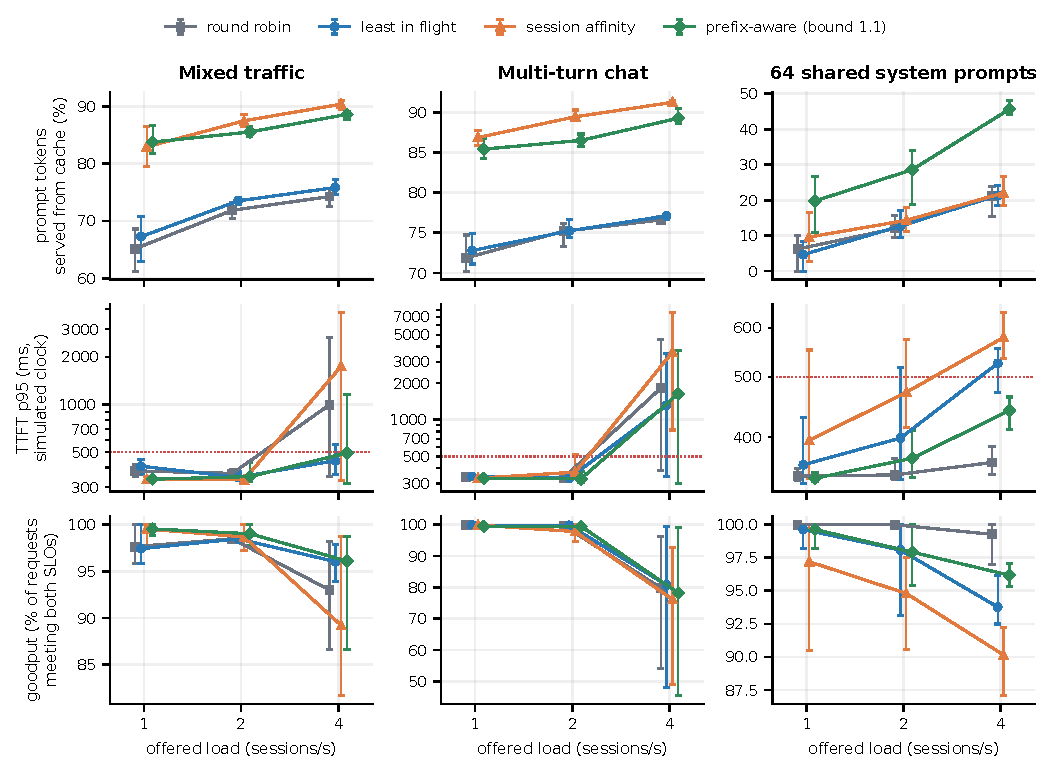
\includegraphics[width=\textwidth]{figures/routing_sweep.pdf}
\caption{Routing strategies across offered load (\Simulated{}; mean of 5 seeds, bars show
the per-seed min--max). Top: share of prompt tokens served from the hosts' prefix caches.
Middle: TTFT p95 on the simulated clock (log scale; dotted line is the 500\,ms SLO). Bottom:
goodput. At 4 sessions/s multi-turn traffic saturates the four hosts on two of five seeds
for every strategy.}
\label{fig:routing}
\end{figure*}

\paragraph{Below saturation.} At 1 and 2 sessions/s (\cref{fig:routing}), prefix-aware
routing reduced median TTFT by 29--39\% relative to least in flight (e.g.\ multi-turn at
1/s: 78 vs.\ 127\,ms; mixed at 2/s: 82 vs.\ 116\,ms) and came within 10\,ms of session
affinity's median. It matched least in flight's p95 within a few milliseconds or improved
on it (mixed at 1/s: 338 vs.\ 407\,ms), with goodput of 99.0--99.5\%. Cache hits rose from
67--76\% (least in flight) to 84--89\% on mixed traffic, against 83--90\% for session
affinity. Round robin tracked least in flight.

\paragraph{At 4 sessions/s.} Means hide per-seed behaviour here. On mixed traffic,
prefix-aware routing had the best p95 on four of five seeds (318--334\,ms against least in
flight's 361--462\,ms, goodput 98--99\% against 96--98\%) but lost the burstiest seed
(1{,}159 vs.\ 558\,ms), which dominates its mean p95 of 494\,ms. Session affinity's mean p95
was 1{,}746\,ms with two seeds near 3--4\,s, because hashing sessions without load placed
more requests on one host than its batch limit admitted (in the pre-change baseline, 192
requests on one host against 128--136 on the others). Multi-turn traffic at 4/s saturated
the fleet on two seeds for every strategy (mean goodput 76--81\%); no routing choice fixes a
fleet that is out of capacity.

\paragraph{Shared prompts beyond one host's cache.} With 64 prompts, a prompt's first use
is always a miss, so the reachable hit rate is about 25\%, 38\% and 58\% at 1, 2 and 4
sessions/s. Prefix-aware routing reached 19.8\%, 28.6\% and 45.7\%, i.e.\ 75--79\% of
reachable; the other strategies reached 4.7--22.1\%, i.e.\ 19--38\%. Median TTFT barely
moved because most requests are first uses. Concentration has a tail cost when most traffic
is cold: at 4/s prefix-aware p95 was 441\,ms against round robin's 364\,ms (least in flight
526\,ms), with goodput 96.2\% against 99.3\% (93.8\%).

\paragraph{Without a session key.} When clients omit the OpenAI \code{user} field, session
affinity has nothing to hash and degenerates to rotation. At 2 sessions/s its cache hits
fell to 75.0\% (multi-turn) and 72.2\% (mixed), with median TTFT 137 and 113\,ms;
prefix-aware routing, which never reads the field, kept 86.4\% and 85.9\% at 88 and 81\,ms.

\begin{figure}[t]
\centering
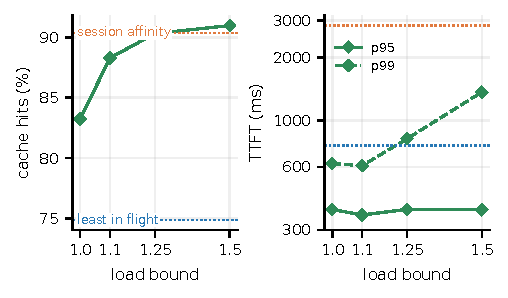
\includegraphics[width=\columnwidth]{figures/routing_bound.pdf}
\caption{Load-bound sensitivity, mixed traffic at 4 sessions/s (\Simulated{}, 5 seeds).
Dotted lines: least in flight (blue) and session affinity (orange); in the right panel
they mark those strategies' mean TTFT p99.}
\label{fig:bound}
\end{figure}

\begin{table}[t]
\centering
\caption{Load-bound sweep, mixed traffic at 4 sessions/s (\Simulated{}, 5 seeds, means).}
\label{tab:bound}
\small
\begin{tabular}{@{}l r r r r@{}}
\toprule
Strategy & \multicolumn{2}{c}{TTFT p50/p95/p99 (ms)} & Hits & Goodput \\
\midrule
least in flight & \multicolumn{2}{r}{136 / 440 / 761} & 74.9\% & 96.1\% \\
session affinity & \multicolumn{2}{r}{95 / 1723 / 2856} & 90.4\% & 90.5\% \\
prefix, $\alpha{=}1.0$ & \multicolumn{2}{r}{110 / 376 / 623} & 83.2\% & 98.2\% \\
prefix, $\alpha{=}1.1$ & \multicolumn{2}{r}{95 / 353 / 608} & 88.3\% & 97.9\% \\
prefix, $\alpha{=}1.25$ & \multicolumn{2}{r}{94 / 376 / 819} & 90.3\% & 97.3\% \\
prefix, $\alpha{=}1.5$ & \multicolumn{2}{r}{92 / 374 / 1368} & 91.0\% & 97.0\% \\
\bottomrule
\end{tabular}
\end{table}

\paragraph{Choosing the bound.} \Cref{fig:bound} and \cref{tab:bound} show the
trade-off the bound controls. A bound of 1.0 is as even as least in flight and gives up
about a third of the available cache benefit. Loosening past 1.1 buys two to three points
of cache hits for a p99 up to 1.8$\times$ worse---the session-affinity failure in
miniature. We chose 1.1 as the default. The corresponding multi-turn sweep was
inconclusive because two of five seeds saturated every strategy.

\paragraph{Threats.} Hosts are simulated, there is one gateway and there are four backends;
the byte-block index only approximates engine token blocks; and some sweeps ran
concurrently, which raised measured gateway overhead (4.4\,ms when run alone, 4.8--5.2\,ms
concurrently). The result is a comparison of strategies under one host model, not a
statement about any GPU.

\subsection{Q2: Agentic correctness}
\label{sec:eval-agents}

\paragraph{Live checks (\PointInTime{}, 16 Nov 2026).} Against a live stamp, the
final-answer format enforcement passed 3 of 3 trials of a request that declared tools and
a JSON schema. An eight-check smoke test using the unmodified OpenAI Agents SDK (token
exchange, model listing, plain chat, a raw tool call with valid JSON arguments, a
multi-tool agent, a handoff between agents, an agent with tools and a typed output, and a
streamed agent run with tool events) passed all eight checks. These are single
observations, not reliability estimates.

\paragraph{A configuration-clock defect seen on the generation clock.} On the same day,
tool-calling requests to a Qwen3.5-2B deployment returned HTTP 400 until a tool-call parser
preset for that model was added to the operator's model profiles; the model host then
restarted in 71\,s and tool calls succeeded. The parser is a configuration-clock setting
(it is fixed at host start), but its absence was visible only as generation-clock errors.
\sys{} now pins exact model-to-parser mappings (Qwen3.5 and Qwen3.6 use an XML tool-call
format, Qwen3-VL a JSON one) and refuses a deployment-supplied parser that contradicts a
model's native template.

\paragraph{Automated tests (\Tested{}).} At the evaluated commit, all Go packages of the
agent, operator and collector pass \code{go test}. The data-plane suite includes tests that
run the real OpenAI Agents SDK against the gateway with a scripted host; guard tests for
repair, failure, billing of discarded attempts and the no-tools final-answer retry; edge
tests for cross-account refusal, connect-only failover, no replay after a request may have
been sent, run-id affinity, serving from the saved table with the control plane down, and a
test that inference through the edge never contacts the control plane; and prefix-routing
tests including a four-turn conversation reaching one host without a session key.
Run on 17 Nov 2026 in a CPU-only container, the data-plane suite reported 785 passed and 2
skipped test cases (parametrized cases counted individually), and the control-plane suite
reported 314 passed and 20 skipped; the skipped cases include tests that need a PostgreSQL
server (among them the row-level-security tests), which this run did not provide.

\subsection{Q3: Heterogeneous bring-up and cold start}
\label{sec:eval-coldstart}

\paragraph{Blackwell stamp (\PointInTime{}, 16 Nov 2026).} A single VM with one NVIDIA RTX
PRO 6000 Blackwell GPU (96\,GiB) was enrolled with the one-command bootstrap and served
Qwen3.6-35B-A3B-FP8 (about 37.5\,GB of weights) with a 64K-token context to Ready; the
model-host image pull took 4\,min~4\,s. The demonstration lineup placed one model per GPU:
Qwen3.5-2B on a T4, Qwen3.5-9B with an 8K context on an A10, and the 35B-A3B FP8 model on
the RTX PRO 6000. We did not measure throughput or latency on these stamps.

\paragraph{Where cold-start time goes (\Measured{}, 6 Oct 2026).} \Cref{fig:coldstart}
decomposes the retained events of one Qwen3.5-0.8B host on an AKS T4 node: 334\,s waiting
for a schedulable GPU, 106\,s pulling an 8.9\,GB image, 111\,s from container start to
loaded weights (weights download itself took 10.8\,s for 1.72\,GiB), 330\,s of engine
profiling, KV allocation and warmup, and 40\,s of frontend warmup until the API listened:
922\,s in total. Qwen3.5-2B and 4B reported 351\,s and 355\,s of engine initialization. An
isolated text-only run on a spare T4 reached \code{/health} in 404\,s, of which 313\,s was
engine warmup; its first request took 6.4\,s and the next two 0.76 and 0.75\,s, because
Triton kernels were JIT-compiled on first use. Node caches and CPU reservations differed
between the two runs, so the difference is not an isolated effect of text-only mode.

\begin{figure}[t]
\centering
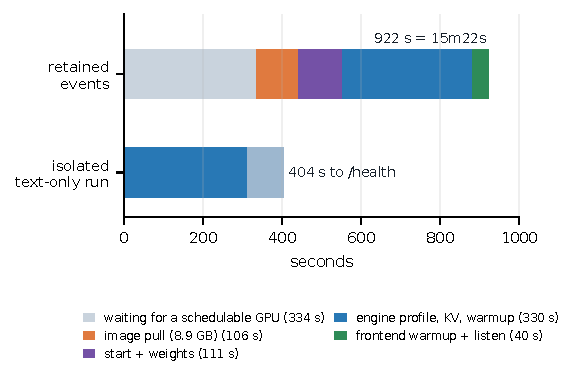
\includegraphics[width=\columnwidth]{figures/cold_start.pdf}
\caption{Configuration-clock cost of one cold T4 model host (\Measured{}, 6 Oct 2026),
from retained timestamps (top) and an isolated text-only validation run measured from
process start (bottom). Weight download is a small fraction; GPU availability and engine
warmup dominate.}
\label{fig:coldstart}
\end{figure}

These data justify two design choices. Rollouts must start a candidate beside the active
release (\cref{sec:config}), because a recreate would expose roughly 15 minutes of
downtime; and placement must refuse what a stamp cannot hold, because a Pending pod's wait
is the single largest stage.

\paragraph{Cloud TPU (\Designed{}).} TPU detection, chart values and the rendered TPU
model host are checked in CI, but vLLM has not been started on TPU chips by us; we make no
TPU serving claim.

\subsection{Q4: Earlier fleet observations}
On 20 Sep 2026 a live audit found five Ready T4 nodes, five Ready model hosts, five
Available one-replica deployments and one HTTP 200 completion from each of five aliases
(\PointInTime{})~\cite{priorpaper}. An earlier two-T4 pilot recorded 30 concurrent requests
under a configured cap producing 5 served and 25 explicit \code{429} refusals with
\code{Retry-After}, all 30 attributed in usage, together with operational anecdotes:
4.25\,GiB of weights loaded from node-local NVMe in 3.3\,s, about 16\,ms per token
single-stream decode, and p95 TTFT near 1.6\,s for that workload (\Measured{}, dated). These
establish reachability and explicit refusal, not throughput, fairness or reliability.

\subsection{What is not evaluated, and the plan}
\label{sec:eval-plan}
We report no hardware throughput or tail-latency results for any current stamp, no
cross-stamp failover measured on production stamps (the edge has run only in a local
two-stamp demonstration with real agents and HTTPS gateways, including serving through a
control-plane outage and an edge restart from cache), no agent task-success rates, and no
TPU results. The evaluation that would close these gaps is: (1) replay the routing
workloads against real vLLM hosts on one GPU class with pinned image, model revision and
settings, reporting engine-side TTFT and time per output token from Prometheus histograms;
(2) run the edge in front of at least two production stamps and inject stamp and
control-plane failures, recording failover latency and the absence of duplicate execution;
(3) measure guard repair rates per model on a public tool-calling benchmark, separating
repaired, failed and valid outcomes and their token cost; and (4) start the TPU path on
v5e and v6e hardware.

% ================================================================= lessons
\section{Lessons}
\label{sec:lessons}

\paragraph{Place state before you route.} Every edge-routing decision we made was forced
by where some piece of generation state lived: run budgets forced strict affinity; prefix
caches allowed soft affinity; stamp-local metering forbade edge metering; stamp-local
cascades limited escalation to one stamp. Writing the state table first
(\cref{tab:state}) would have produced the edge design directly.

\paragraph{Configuration surfaces leak into generation correctness.} Two of our agentic
failures were configuration interactions, not model failures: a missing tool-call parser
(HTTP 400 until the host restarted with the right preset) and an engine that ignores a
requested output format while tools are offered. Both are invisible to the control plane
and visible only on the request path, which argues for gateway-level validation that turns
silent semantic errors into bounded, metered, observable retries.

\paragraph{Charge for corrections.} A guard that re-asks a model hides cost unless it bills
it. Recording discarded attempts as usage, debiting them from rate limits and run budgets,
and reporting attempts in headers kept the mechanism honest and let budgets stop runaway
repair loops.

\paragraph{Outbound-only observation is sufficient.} Status, activity, metrics and logs
pushed by the agent gave the console a complete view of stamps on VMs the central
Prometheus cannot reach, without opening an inbound path. Bounded buffers with event
identifiers made disconnection a delay rather than a loss.

\paragraph{Cold start is a scheduling resource.} Image pulls, engine warmup and GPU
availability make minutes of configuration-clock time per host. Treating spare capacity and
warm caches as resources is a prerequisite for safe rollouts and for any autoscaler.

% ================================================================= limitations
\section{Limitations and Threats to Validity}
\label{sec:limits}

\paragraph{Evidence.} The routing results use simulated hosts. Live checks are single
observations without repetition or confidence intervals. The September audit, the October
validation and the November checks differ in topology and software. The bring-up of the
Blackwell stamp establishes that the path works once, not its reliability.

\paragraph{Known gaps.} The stamp pod still mounts the agent's Kubernetes service-account
token into the gateway and collector containers, so I1 is enforced by application roles
but not by Kubernetes credentials. The September analysis also reported a same-release
replica reduction that did not converge automatically and a one-pass reconciliation delay
after projected-token rotation~\cite{priorpaper}; we have not re-audited either. Limits,
runs and prefix indexes are per stamp or per gateway process, not global; an account served
by two stamps can use both stamps' allowances. Agent runs are in memory and lost on gateway
restart. The edge's routing-table credential, if leaked, exposes every account's deployment
and placement metadata (but no prompts or secrets). The tool-call guard checks only
non-streaming chat completions. Usage records are operational, not billing-grade. Hosted
code execution in the process sandbox shares a kernel across runs unless a gVisor or Kata
runtime class or microVM backend is configured. GPU sharing is designed but not
implemented, so large GPUs serving moderate models are underused.

\paragraph{Kernel work.} A fused decode-step kernel for the gated-delta recurrence was
measured at 1.81$\times$ the stock operation at batch 1 inside a CUDA graph on T4 (20.37
vs.\ 11.30\,$\mu$s) with bit-identical outputs, reaching parity at 16--32 sequences
(\DevOnly{}). The operation is roughly 2\% of a token's cost, it is not enabled in serving,
and we claim no end-to-end benefit.

% ================================================================= conclusion
\section{Conclusion}
\label{sec:conclusion}
A managed LLM service is easier to reason about as two clocks than as one control loop.
Extending \sys{} with an edge tier, cache-aware routing, heterogeneous stamps and agentic
requests added state at every tier; the rule that state lives with the clock that reads it
told us where each piece belonged and what affinity, retry and metering behaviour the
routers in front of it must provide. The resulting system serves one endpoint across stamps
without putting the control plane on the request path, routes for cache reuse without
session affinity's tail, and governs agent loops with budgets, content-free traces and
honest, bounded repair of the tool-call and output-format errors that small open models
make. Its evidence is uneven, and we have classified it accordingly: a simulated routing
study, dated cold-start records, and point-in-time live checks, with throughput on real
hardware, production edge failover and TPU serving left as stated future work.

\section*{Acknowledgements}
[To be added.]

\balance
\bibliographystyle{plain}
\bibliography{references}

\appendix
\section{Reproducibility and Evidence Map}
\label{app:repro}
Source code and records: \repourl, commit \code{018b56e}. All plotted values are read
from the repository: \code{paper/data/evidence.json} (evidence register, including the
16~November live observations with scope ``point-in-time live check'' and the 6~October
cold-start timestamps) and the routing artifacts under
\code{docs/benchmarks/routing-2026-11-05/} (schema \code{fabric.routing-benchmark/v1}; each
records its command, commit, dirty flag, host model and per-seed summaries). Figures are
regenerated deterministically with
\code{uv run --project paper python paper/generate\_figures.py}; the routing benchmark is
rerun with \code{make bench-routing}. The edge, agent-loop, cascade and agent-run
demonstrations run without a GPU via \code{make demo-edge}, \code{make demo-agent-loop},
\code{make demo-cascade} and \code{make demo-agent}. Operational identifiers (hostnames,
cloud resource names, addresses, credentials) are omitted from this paper by design.

\end{document}
